\chapter{Generování geometrie}\label{geometrie}
V této práci budeme v rámci všech numerických simulací předpokládat rigidní geometrii. To umožní před spuštěním numerické simulace vygenerovat všechny potřebné objekty, které lze během numerické simulace použít. Konkrétně je mimo jiné možné před začátkem numerických výpočtů určit, v jakých bodech diskrétní mřížky se bude nacházet překážka, vypočítat hodnoty parametru $ \Theta $ ze sekce \ref{interpolation bc} a určit tvary normálových vektorů v bodech, které jsou použity pro výpočet síly, jak bylo popsáno v~sekci~\ref{vypocet sily v LBM}.

V této sekci popíšeme použitý proces generování geometrie použitý v rámci této práce. Jelikož k numerickým simulacím využita mřížková Boltzmannovu metoda (viz kapitola \ref{lbm}), je tomu proces generování geometrie uzpůsoben a jeho cílem je připravit data tak, aby pak mohla být vhodně využita v rámci diskrétní ekvidistantní mřížky použité v LBM. 

\section{Struktura generovaných dat}\label{struktura dat}
Výsledná vygenerovaná geometrie je na závěr exportována jako datový soubor, který lze v rámci numerické simulaci načíst. Nejdříve tedy popíšeme strukturu exportovaného souboru. Jak již bylo zmíněno, hlavním cílem generátoru je popsat jednotlivé body mřížky použité v LBM.

U každého bodu mřížky lze jednoznačně určit jeho souřadnice na mřížce a zda se v něm nachází překážka. Dále můžeme v každém bodu určit hodnoty interpolačních parametrů $ \Theta $ pomocí \eqref{eq:q} - pokud se v okolí bodu v daném směru nenachází hranice žádného objektu, definujeme z implementačních důvodů hodnotu přílušného interpolačního parametru jako $ -1$. Výpočet interpolačního parametru bude podrobněji rozebrán později.

V každém z bodů můžeme tedy určit souřadnice $ x $ a $ y $, informaci o přítomnosti překážky a dále celkem 8 různých hodnot interpolačního parametru. Při použití diskrétní mřížky ve tvaru \eqref{eq:oblast} exportovaný soubor tedy obsahuje matici rozměru $ c \times 11$, kde $ c $  označuje kardinalitu množiny $ \hat{\Omega} $ z \eqref{eq:oblast}.

Podotkněme, že pokud je předmětem zkoumání síla působící na obtékaný objekt, je nutné mimo právě popsaný exportovaný soubor předat dále také pole obsahující informaci o normálových vektorech v lagrangeovských bodech, které diskretizují hranici objektu. Výpočet normálových vektorů na hranici je podorobněji popsán dále. Jelikož v této práci není zkoumáno silové působení, uvažujeme pouze export souboru popsaného výše.

\section{Výpočet normálového vektoru}
V případě, kdy je přímo zadán analytický předpis hranice diskretizovaného objektu, lze hodnoty normálového vektoru v každém z bodů diskretizujících hranici jednoduše nalézt pomocí metod matematické analýzy. Pokud nemáme k dispozici analytický popis hranice, můžeme hranici po částech lineárně aproximovat spojením sousedních lagrangeovských bodů úsečkou. Normálové vektory v jednotlivých bodech pak můžeme aproximovat průměrem normálových vektorů ze sousedních bodů. Schematicky je tato konstrukce vyobrazena na obr. \ref{fig:aproximace hranice}.


\begin{figure}[H]
	\centering
	\vspace{2.8mm}
	\includegraphics[width=0.7\textwidth, trim={7.9cm 1.6cm 0cm 0cm}]{Images/lincurve.pdf}
	\vspace{1.8mm}
	\caption{Ilustrace konstrukce normálových vektorů u obecné křivky bez zadaného analytického předpisu. $ \boldsymbol{X} $ představuje jeden z lagrangeovských bodů diskretizujících hranici. Tvar hranice, která je po částech lineárně nahrazena, je znázorněn čárkovaně.}
	\label{fig:aproximace hranice}
	\vspace{0mm}
\end{figure}


\section{Výpočet interpolačního parametru}
Pro výpočet interpolačního parametru $ \Theta $ nyní opět předpokládejme, že máme k dispozici analytický popis křivky popisující hranici nebo využijeme již zmíněné po částech lineární aproximace. To jednoznačně určuje vazbu $ \phi = 0$ určující tvar spojité hranice objektu.

Parametr $ \Theta $ je nutné vypočítat pro každý ze směrů možného šíření kromě směru odpovídajícímu $ \vec{\xi}_0 $. V rámci modelu D2Q9 tedy celkem určujeme 8 hodnot pro každý bod hranice, označme je $ \Theta_1, \Theta_2, \dots, \Theta_8$, kde číslo indexu odpovídá příslušnému směru, viz obr. \ref{fig:d2q9}. Použijeme-li značení z obr. \ref{fig:bouz}, tak lze nahlédnout, že průsečík $ \vec{x}_w $ s hranicí nemůže existovat pro každý ze směrů. Jak již bylo zmíněno, z implementačních důvodů pro směry, ve kterých nenajdeme průsečík s hranicí, pokládáme  $ \Theta_i = -1$, přičemž Bouzidiho interpolační podmínka popsaná v sekci \ref{interpolation bc} v těchto směrech není použita.

Interpolační parametr získáme vypočtením průsečíku hranice a úsečky ve směru $ \vec{\xi}_i $. Opět s použitím značení z obr. \ref{fig:bouz} parametrizujme úsečku spojující body $ \vec{x}_{f{_A}} = (x_{f{_A}}, y_{f{_A}})$ a $ \vec{x}_b  = (x_b, y_b)$ jako
\begin{align}\label{eq:parametrizace usecky}
\begin{split}
x=& s \, x_{f{_A}} + (1 - s) \, x_b,
\\
y=& s \, y_{f{_A}} + (1 - s) \, y_b ,
\end{split}
\end{align}
kde $ s \in \langle 0, 1 \rangle $. Dále dosazením \eqref{eq:parametrizace usecky} do rovnice vazby $ \phi $ získáme obecně nelineární rovnici pro $ s $. Tuto rovnici řešíme v rámci generátoru pomocí Powellovy hybridní metody \cite{Powell}, která je dostupná v rámci knihovny SciPy implementované v jazyce Python. Je snadné nahlédnout, že získaná hodnota $ s $ pak odpovídá hledané hodnotě parametru $ \Theta_i $, a není tedy nutné explicitně počítat souřadnice bodu  $ \vec{x}_w $ a používat vztah \eqref{eq:q}. Podotkněme, že v rámci tohoto kroku předpokládáme, že řešení výše zmíněné nelineární rovnice bude nejvýše jedno, což však nepředstavuje výrazné omezení pro tvary objektů, které můžeme použít.

\section{Struktura kódu a poznámky k implementaci}\label{meshgenenator}
Generátor 2D geometrie použitý v rámci této práce byl objektově implementovaný v programovacím jazyce Python s využitím volně dostupných knihoven. Celý generátor tvoří samostatný balík jménem \texttt{meshgenerator}. V této sekci krátce popíšeme strukturu a fungování tohoto balíku sestávajícího ze tří hlavních částí. Struktura a propojení tříd v rámci balíku \texttt{meshgenerator} je znázorněna na obr. \ref{fig:uml meshgenerator}.

První část obsahuje pomocné funkce a pomocnou třídu \texttt{Point}, která rezprezentuje jeden bod na mřížce, tedy mezi její atributy patří souřadnice, informace o přítomnosti překážky a hodnoty interpolačních parametrů.

Druhá část se skládá z jednotlivých modulů, které obsahují třídy a podtřídy reprezentující jednotlivé objekty, které lze v rámci simulace použít. Potomkem rodičovské třídy \texttt{GeneralObject}, která zastřešuje veškeré použitelné objekty, je třída \texttt{ClosedObject}, resp. \texttt{OpenObject},  reprezentující objekty s definovaným vnitřkem, resp. objekty bez jednoznačně definovaného vnitřku. Třída \texttt{OpenObject} tedy navíc obsahuje atribut nesoucí informaci o orientaci objektu v oblasti, díky němuž lze pak jednoznačně objekt vymezit. Ze třídy \texttt{ClosedObject} jsou pak dále odvozené třídy \texttt{Polygon} (reprezentuje objekty ve tvaru mnohoúhelníka) a \texttt{Implicit} (reprezentuje objekty, které jsou definovány pomocí implicitního vztahu). Pro následné zjednodušení práce s konkrétními implicitně zadanými objekty byly definovány třídy \texttt{Circle} (reprezentuje objekty ve tvaru kružnice), \texttt{Ellipse} (reprezentuje objekty ve tvaru elipsy) a \texttt{CassiniOval} (reprezentuje objekty ve tvaru Cassiniho oválu\footnote{Cassiniho ovál je křivka pojmenovaná po Giovannim Cassinim. Jsou-li $ P_1 $ a $ P_2 $ dva pevné body v rovině a $ b > 0$, pak je Cassiniho ovál formálně definován jako množina $$ \left\{ \, P \: \big| \: |PP_1|\cdot|PP_2| = b^2 \, \right\} ,$$ tedy množinou bodů, jejichž součin vzdáleností od $ P_1 $ a $ P_2 $ je konstantní.}) Ze třídy \texttt{OpenObject} jsou odvozené třídy \texttt{FunctionCurve} (reprezentuje objekty zadané pomocí explicitního funkčního předpisu) a \texttt{SVGCurve} (reprezentuje křivku, která byla vytvořena ve formátu $\mathtt{SVG} $ \cite{Eisenberg2002}). Pro případné jednodušší generování zúžených cév pak byla implementována třída \texttt{Exponential}, která je potomkem třídy \texttt{FunctionCurve}. Model stenózy cévy vzniklý použitím instancí třídy \texttt{Exponential} je prezentován na obr. \ref{fig:vessel exponential}. Podotkněme, že všechny implementované objekty byly vybrány tak, aby byly lehce popsatelné pomocí několika parametrů a byly tak vhodné pro využití v rámci optimalizace, která je předmětem této práce. Výjimku tvoří třída \texttt{SVGCurve}, která vznikla v rámci předchozí bakalářské práce a která nevyužívá k vytvoření objektu žádného parametru a nelze ji tak v rámci optimalizace použít.


\begin{figure}[h]
	\centering
	\vspace{8mm}
	\includegraphics[width=0.95	\textwidth]{Images/figvessel.pdf}
	\vspace{2mm}
	\caption{Model stenózy cévy vzniklý použitím instancí třídy \texttt{Exponential}.}
	
	\label{fig:vessel exponential}
	\vspace{1.8mm}
\end{figure}

Třetí část balíku \texttt{meshgenerator} pak definuje třídu \texttt{NumSimProblem}, která souhrnně definuje celou úlohu, jež je dále numericky řešena. Pomocí konfiguračního souboru, v kterém jsou definovány uživatelem požadované parametry výpočetní oblasti, je inicializována datová struktura popsaná v sekci \ref{struktura dat} obsahující veškeré body diskrétní mřížky použité v LBM. Konstruktoru třídy \texttt{NumSimProblem} jsou dále předány všechny instance podtříd třídy \texttt{GeneralObject}, které tvoří celkovou požadovanou geometrii a které jsou dále využity pro aktualizaci informací o jednotlivých bodech mřížky. Vygenerovaná datová struktura je pak exportována a dále využita v rámci numerické simulace.

\begin{figure}[h]
	\centering
	\vspace{8mm}
	\includegraphics[width=0.9	\textwidth]{Images/umldiagram.pdf}
	\vspace{2mm}
	\caption{Diagram znázorňující strukturu a využití tříd v rámci balíku \texttt{meshgenerator}.}
	\label{fig:uml meshgenerator}
	\vspace{1.8mm}
\end{figure}